% VLDB template version of 2020-08-03 enhances the ACM template, version 1.7.0:
% https://www.acm.org/publications/proceedings-template
% The ACM Latex guide provides further information about the ACM template

\documentclass[sigconf, nonacm]{acmart}

%% The following content must be adapted for the final version
% paper-specific
\newcommand\vldbdoi{XX.XX/XXX.XX}
\newcommand\vldbpages{XXX-XXX}
% issue-specific
\newcommand\vldbvolume{14}
\newcommand\vldbissue{1}
\newcommand\vldbyear{2021}
% should be fine as it is
\newcommand\vldbauthors{\authors}
\newcommand\vldbtitle{\shorttitle} 
% leave empty if no availability url should be set
\newcommand\vldbavailabilityurl{http://vldb.org/pvldb/format_vol14.html}
% whether page numbers should be shown or not, use 'plain' for review versions, 'empty' for camera ready
\newcommand\vldbpagestyle{plain} 

\usepackage{caption}
\usepackage{subcaption}
\usepackage{multirow}

\usepackage{booktabs} % For formal tables


\newlength\Origarrayrulewidth

% horizontal rule equivalent to \cline but with 2pt width
\newcommand{\Cline}[1]{%
	\noalign{\global\setlength\Origarrayrulewidth{\arrayrulewidth}}%
	\noalign{\global\setlength\arrayrulewidth{3pt}}\cline{#1}%
	\noalign{\global\setlength\arrayrulewidth{\Origarrayrulewidth}}%
}

% draw a vertical rule of width 2pt on both sides of a cell
\newcommand\Thickvrule[1]{%
	\multicolumn{1}{!{\vrule width 2pt}c!{\vrule width 2pt}}{#1}%
}

% draw a vertical rule of width 2pt on the left side of a cell
\newcommand\Thickvrulel[1]{%
	\multicolumn{1}{!{\vrule width 2pt}c}{#1}%
}

% draw a vertical rule of width 2pt on the right side of a cell
\newcommand\Thickvruler[1]{%
	\multicolumn{1}{c!{\vrule width 2pt}}{#1}%
}


\begin{document}
\title{Context-Free Path Querying In Terms of Linear Algebra}

%%
%% The "author" command and its associated commands are used to define the authors and their affiliations.
\author{Rustam Azimov \\ supervised by Semyon Grigorev} 
\affiliation{%
  \institution{Saint Petersburg State University}
  \streetaddress{7/9 Universitetskaya nab.}
  \city{St. Petersburg}
  \state{Russia}
  \postcode{199034}
}
\email{st013567@student.spbu.ru}

%%
%% The abstract is a short summary of the work to be presented in the
%% article.
\begin{abstract}
Context-Free Path Querying (CFPQ) is an important problem with applications in many areas, for example, graph databases, bioinformatics, static analysis, etc. Historically, regular languages are used as constraints for
navigational path queries. However, in some important cases, regular languages are not expressive enough and context-free languages are used instead. Many algorithms for CFPQ were proposed but recently showed
that the state-of-the-art CFPQ algorithms are still not performant enough for practical use. One promising way to achieve
high-performance solutions for graph querying problems is to
reduce them to linear algebra operations (such as matrix
multiplication). The active utilization of these operations in the process of context-free path query evaluation
makes it possible to efficiently apply a wide class of optimizations
and computing techniques, such as GPGPU (General-Purpose computing on Graphics Processing Units), parallel computation, sparse
matrix representation, distributed-memory computation, etc. In this Ph.D. work, we aim at: (i) studying the applicability of linear algebra methods to the CFPQ problem, (ii) at devising the algorithms for context-free path query evaluation formulated in terms of linear algebra operations, and (iii) at achieving high-performance implementations of the devised algorithms using parallel computations.
\end{abstract}

\maketitle

%%% do not modify the following VLDB block %%
%%% VLDB block start %%%
\pagestyle{\vldbpagestyle}
%\begingroup\small\noindent\raggedright\textbf{PVLDB Reference Format:}\\
%\vldbauthors. \vldbtitle. PVLDB, \vldbvolume(\vldbissue): \vldbpages, \vldbyear.\\
%\href{https://doi.org/\vldbdoi}{doi:\vldbdoi}
%\endgroup
\begingroup
\renewcommand\thefootnote{}\footnote{\noindent
Proceedings of the VLDB 2021 PhD Workshop, August 16th, 2021. Copenhagen, Denmark. Copyright (C) 2020 for this paper by its authors. Use permitted under Creative Commons License Attribution 4.0 International (CC BY 4.0). \\
}\addtocounter{footnote}{-1}\endgroup
%%% VLDB block end %%%

%%% do not modify the following VLDB block %%
%%% VLDB block start %%%
%\ifdefempty{\vldbavailabilityurl}{}{
%\vspace{.3cm}
%\begingroup\small\noindent\raggedright\textbf{PVLDB Artifact Availability:}\\
%The source code, data, and/or other artifacts have been made available at %\url{\vldbavailabilityurl}.
%\endgroup
%}
%%% VLDB block end %%%

\section{Introduction}

\begin{figure*}[t]
	\centering
	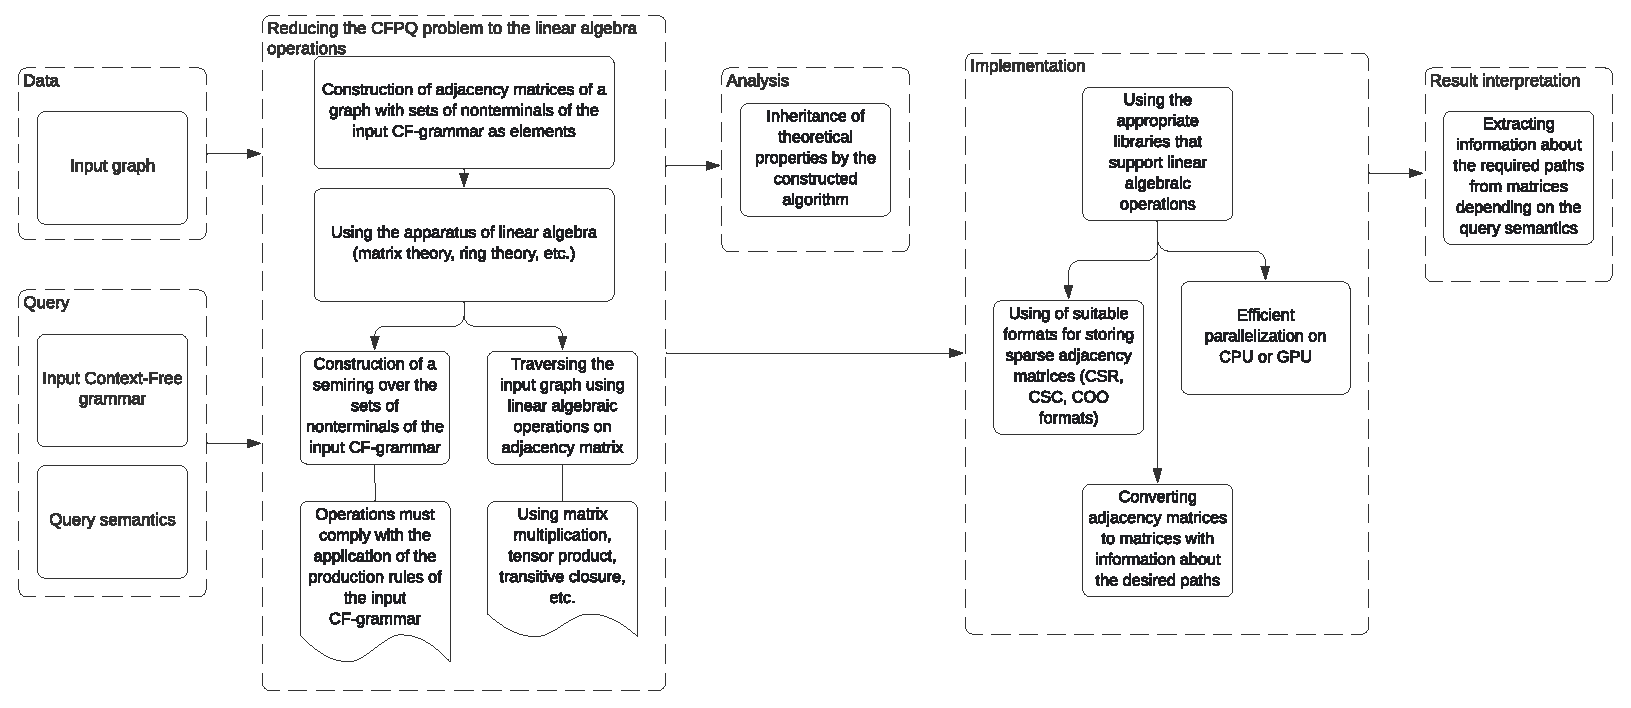
\includegraphics[width=\linewidth]{figures/schema eng.pdf}
	\caption{An overview of our proposed approach to solving the CFPQ problem using linear algebra operations}
	\label{fig:schema}
\end{figure*}

Formal language-constrained path querying~\cite{doi:10.1137/S0097539798337716} is a graph analysis problem in which formal languages are used as constraints for
navigational path queries. In this problem, a path in an edge-labeled graph is viewed
as a word constructed by the concatenation of edge labels. The formal languages are used to constrain the paths of interest: a query should find only paths labeled by words from the language. The most popular class of constraints used as navigational queries in graph databases are the regular ones.
However, in some important cases, regular languages are not expressive enough and context-free languages are used instead. The context-free path querying (CFPQ), can be used in many areas, for example, RDF analysis~\cite{10.1007/978-3-319-46523-4_38}, static code analysis~\cite{Zheng,10.1145/373243.360208}, biological data analysis~\cite{SubgraphQueriesbyContextfreeGrammars}, graph segmentation~\cite{8731467}.

CFPQ has been studied a lot since the problem was first stated by Mihalis Yannakakis in 1990~\cite{Yannakakis}.
Jelle Hellings investigates various aspects of CFPQ in~\cite{hellingsPathQuerying,hellingsRelational,DBLP:journals/corr/Hellings15} and formulates three possible querying semantics: \textit{relational} that requires to find all vertex pairs reachable by some path of interest, \textit{single-path} query semantics also requires to return the example of such path for all vertex pairs, and \textit{all-path} query semantics that requires to return all such paths for all vertex pairs.

A number of CFPQ algorithms based on parsing techniques were proposed: (G)LL and (G)LR-based algorithms by Ciro M. Medeiros et al.~\cite{Medeiros:2018:EEC:3167132.3167265}, Fred C. Santos et al.~\cite{10.1007/978-3-319-91662-0_17}, Semyon Grigorev et al.~\cite{Grigorev:2017:CPQ:3166094.3166104}, and Ekaterina Verbitskaia et al.~\cite{10.1007/978-3-319-41579-6_22}; CYK-based algorithm by Xiaowang Zhang et al.~\cite{10.1007/978-3-319-46523-4_38}; combinators-based approach to CFPQ by Ekaterina Verbitskaia et al.~\cite{Verbitskaia:2018:PCC:3241653.3241655}.
Yet recent research by Jochem Kuijpers et al.~\cite{Kuijpers:2019:ESC:3335783.3335791} shows that existing solutions are not applicable for real-world graph analysis because of significant
running time and memory consumption.

Inspired by Valiant's~\cite{valiant} matrix-based algorithm for context-free language recognition, we explore the applicability of linear algebra methods to the CFPQ problem. The linear algebra methods is widely used for various problems of finding paths in graphs, but the CFPQ problem poses additional challenges originating from query-specific information that needs to be captured. Valiant proposed a parsing algorithm, which computes a recognition table by computing matrix transitive closure. These algorithms take a string
at the input and decide whether this string is generated from the
input context-free grammar. Valiant’s algorithm has essentially the same complexity as Boolean matrix multiplication. This is a promising way to achieve high-performance solutions for graph querying problems. The active utilization of these operations in the process of context-free path query evaluation
makes it possible to efficiently apply a wide class of optimizations
and computing techniques, such as GPGPU (General-Purpose computing on Graphics Processing Units), parallel computation, sparse
matrix representation, distributed-memory computation, etc.

In this Ph.D. work, we make the following contributions.
\begin{enumerate}
	\item We provide an approach to solving the CFPQ problem using linear algebra operations. The provided approach allows us to use a wide class of optimizations of linear algebra operations for efficient analysis of large graphs.
	
	\item Using provided approach, we devise the CFPQ algorithms based on linear algebra operations for relational, single-path, and all-path query semantics.
	
	\item We provide the implementations of the devised algorithms for context-free path query evaluation using different optimizations	and computing techniques. Our preliminary results demonstrate that our best CPU and GPU-based implementations that utilize sparse matrix representation and parallel computation outperform the state-of-the-art context-free path querying solutions.
\end{enumerate}

\section{Approach}

In this section, we describe our approach to solving the CFPQ problem using linear algebra operations. The idea of using a sparse adjacency matrix as a graph representation in graph analysis problems is well-known. Recently, became very popular the GraphBLAS~\cite{7761646} API specification that defines standard building blocks for graph algorithms in the language of linear algebra. Various libraries that implement it provide data structures and functions to compute linear transformations and other linear algebra operations on sparse matrices. Using these libraries or other efficient libraries for such operations is a good recipe for making a high-performance CFPQ solution if we can reduce the CFPQ problem to linear algebra operations. Although such reduction was found for a number of graph algorithms, there are many graph algorithms for which it has not been done. To the best of our knowledge, the reduction of CFPQ problem to linear algebra operation is an open question.

An overview of our proposed approach is shown in \autoref{fig:schema}. The purpose of this approach is to solving CFPQ problem using linear algebra operations. In order to do this, it is necessary to devise the CFPQ algorithms that have the input in the form of a directed edge-labeled graph as a data, a context-free grammar as a query, and the query semantics that determines the type of requested information about paths in the graph. Further, the approach can be divided into the following stages.

\paragraph{Reducing the CFPQ problem to the linear algebra operations} 
The query is formulated by a \emph{context-free grammar} $G$ which is a tuple $(N, \Sigma, P, S)$, where $N$ is a finite set of nonterminals; $\Sigma$ is a finite set of terminals, $N \cap \Sigma = \varnothing$; $P$ is a finite set of productions of the form $A \to \alpha$, where $A \in N,\ \alpha \in (N \cup \Sigma)^*$; and $S$ is the start nonterminal. To formulate the obtained problem in terms of linear algebra, the input graphs are considered in the form of adjacency matrices, and the input context-free grammar (CF-grammar) is encoded in the form of a certain algebraic structure, namely, in the form of a semiring with non-associative multiplication. This approach takes advantage of the fact that in the production rules of the CF-grammars there are two operations --- concatenation and union, which are transformed into the product and the sum of a semiring. The elements of the adjacency matrices must be sets of nonterminals since each of them describe the set of words corresponding to the paths of interest. Further, the resulting semiring is used to define matrix multiplication (or other linear algebra operation), which simulates the step of the input graph traversing. For a complete traversal of the input graph, a transitive closure of adjacency matrices can be defined, which allows us to obtain the information about all paths corresponding to the query. The type of information retrieved depends on the query semantics, which must be taken into account when constructing the adjacency matrices and semirings.


\paragraph{Analysis}
To analyze the theoretical properties of the constructed algorithm, the existing theoretical results of linear algebra, graph theory and the theory of formal languages can be used. The properties of the entire CFPQ algorithm largely depend on the properties of linear algebra operations since it evaluates the context-free path queries by offloading the most intensive computations into calls
to procedures for these operations. Therefore, the most effective for the algorithm will be optimizations that use the existing results of linear algebra to efficiently compute such operations, for example, sparse matrix and vector operations.

\paragraph{Implementation}
From a practical point of view, the algorithms built in this approach are easy to implement, since the most time consuming is the implementation of the necessary linear algebra operations, which have already been implemented in many efficient libraries that support linear algebra operations. For example, can be used the SuiteSparse:GraphBLAS~\cite{Davis2018Algorithm9S} library --- is an implementation of the GraphBLAS API. In such libraries, various matrix optimizations are used, which will significantly speed up the computation of the context-free queries for large graphs. One of such optimizations is the use of sparse matrix formats (CSR, CSC, COO), the use of which gives a significant performance gain since real data is often sparse. In addition, many linear algebra operations can be efficiently computed in parallel, for example on a GPU. As a result, the CFPQ implementation will allow to obtain matrices that will store information about the desired paths in the graph. The type of stored information is determined by the query semantics, for example, it can be an answer to the question of the existence of paths of a certain form or their enumeration.

\paragraph{Result interpretation} 
The final step is to interpret the query result. Depending on the query semantics, it is possible to extract certain information about the paths between the vertices of interest from the resulting matrix. In addition, in the case when the query semantics involves the enumeration of paths between certain vertices in the graph, it also becomes necessary to implement an algorithm for constructing these paths from the resulting matrices.

%To sum up, the novelty of the presented approach is as follows.
%\begin{enumerate}
%\item The currently existing approaches to computing context-free path queries to graphs either do not use linear algebra operations or are intended only for a particular case of CF-grammars and/or specialized graphs.
%\item The proposed approach allows using a wide class of optimizations of linear algebra operations for efficient analysis of large graphs.
%\item The proposed approach allows one to build algorithms that are easy to implement, portable, and makes it possible to easily and efficiently apply parallel computations.
%\end {enumerate}

\section{Algorithms}
 In this section, we briefly describe our devised CFPQ algorithms based on the linear algebra operations. For all our algorithms we formally prove the correctness, termination, and time complexity bounds. Our algorithms can be divided into two groups.
 
 \paragraph{Matrix-based algorithms}
 The algorithms in the first group utilize the Boolean matrix multiplication for relational query semantics and operate with more complex matrices for single-path and all-path query semantics. Also, these algorithms, like many existing ones, require the CF-grammar transformation to some normal form that allows us to encode one step of the input graph traversing into exactly one matrix multiplication since in this form we have only two nonterminals in the right-hand side of productions rules.
 
We define a binary operation $(~\cdot~)$ for arbitrary subsets \mbox{$N_1, N_2$} of $N$ with respect to a CF-grammar \mbox{$G = (N, \Sigma, P)$} as
$$N_1 \cdot N_2 = \{A~|~\exists B \in N_1, \exists C \in N_2 \text{ such that }(A \rightarrow B C) \in P\}.$$

Using this binary operation as subset multiplication, and union as an addition, we can define a \emph{matrix multiplication}, \mbox{$a \times b = c$}, where $a$ and $b$ are matrices of a suitable size, that have subsets of $N$ as elements, as $c_{i,j} = \bigcup^{n}_{k=1}{a_{i,k} \cdot b_{k,j}}$. Also, we use the element-wise union operation on matrices $a$ and $b$ with the same size: \mbox{$a \cup b = c$}, where $c_{i,j} = a_{i,j} \cup b_{i,j}.$ Finally, we define the \emph{transitive closure} of a square matrix $a$ as \mbox{$a^+ = a^{(1)}_+ \cup a^{(2)}_+ \cup \cdots$}, where \mbox{$a^{(1)}_+ = a$} and $a^{(i)}_+ = \bigcup^{i-1}_{j=1}{a^{(j)}_+ \times a^{(i-j)}_+}, ~i \ge 2$.

We can evaluate the context-free path queries with relational semantics by computing this transitive closure of an adjacency matrix $T$ of input labeled graph with sets of nonterminals as elements where $A \in T_{i,j}$ only if there is $x \in \Sigma$ such that there is edge from vertex $i$ to $j$ labeled by $x$ and $(A \rightarrow x) \in P$. However, described operations can be computed using several Boolean matrix multiplications and additions if we encode the matrix $T$ by the $|N|$ Boolean matrices (one Boolean matrix for each nonterminal 
how it is done in the work of Valiant~\cite{valiant}).

For single-path and all-path query semantics, we store additional information in matrices to be able to restore found paths. For single-path query semantics, we store the intermediate vertex $k$ in the element $T_{i,j}$ only if there is a path from $i$ to $k$ corresponding to the nonterminal $B$, there is a path from $k$ to $j$ corresponding to the nonterminal $C$, and there is a rule $(A \rightarrow B C) \in P$. For all-path query semantics, we store the sets of the intermediate vertices, since we must store the information about all paths between each vertex pair. In that case, we cannot reduce computations to operations on Boolean matrices and we use custom matrix multiplication for matrices with more complex elements (tuples or arrays of integers). There are still libraries that support linear algebra operations for our algorithms for single-path and all-path query semantics, for example, the GraphBLAS implementations that support the creation of custom semirings for the matrix operations.

\paragraph{Kronecker product-based algorithm}
On the contrary, the algorithm in the second group is based on the Kronecker product operation and does not require the transformation of the input grammar. The transformation leads to at least a quadratic blow-up in
grammar size, thus by avoiding the transformation, this algorithm achieves better time complexity in terms of the grammar size. While regular languages can be expressed as a Finite-State Machine (FSM), a CF-grammar can be expressed as a Recursive State Machine (RSM) in a similar
fashion. In these algorithms, we use RSM to represent the context-free path query and evaluate this query using the Kronecker product of the corresponding adjacency matrices of the input graph and the RSM for the input CF-grammar. Although the Kronecker-based algorithm for constructing the matrices with information about required paths (or so-called \textit{index}) is the same for all three query semantics, the paths extraction algorithm for each semantics is different.

\section{Preliminary results}
{\setlength{\tabcolsep}{0.4em}
	\begin{table*}[ht]
		\caption{Index creation time for RDFs (time is measured in seconds and memory is measured in megabytes)}
		\label{tbl:tableRDFQ1}
		\begin{tabular}{| l | c | c | r  r | r  r | r  r | r  r |}
			\hline
			
			\multirow{3}{*}{Name}  & \multirow{3}{*}{V} & \multirow{3}{*}{E} & \multicolumn{4}{|c|}{Relational semantics index}	&	\multicolumn{4}{|c|}{Single-path semantics index} \\
			\cline{4-11}
			& & &	\multicolumn{2}{|c|}{RG\_CPU\textsubscript{rel}}	&	\multicolumn{2}{|c|}{RG\_GPU\textsubscript{rel}} &	\multicolumn{2}{|c|}{RG\_CPU\textsubscript{path}}	&	\multicolumn{2}{|c|}{RG\_GPU\textsubscript{path}}	 \\
			\cline{4-11}
			&  & &  Time (s)     & Mem (MB) & Time (s)     & Mem (MB)  &  Time (s)     & Mem (MB) & Time  (s)   & Mem (MB) \\
			\hline
			\hline
			%core                        & 1 323  & 8 684  & 0.004 & 0.3   & 0.010  & 0.1      & 0.002 & 0.3  & 0.016 & 0.1  \\
			go-hierarchy                & 45 007  & 1 960 436 & 0.091 & 16.3 & 0.108 & 121.2    & 0.976 & 92.0   & 0.336 & 125.0  \\
			enzyme                      & 48 815  & 219 390  & 0.018 & 5.9 & 0.018 & 4.0        & 0.029 & 8.1  & 0.043 & 6.0    \\	
			eclass\_514en                 & 239 111  & 1 047 454 & 0.067 & 13.8  & 0.166 & 16.0     & 0.195 & 31.2 & 0.496 & 26.0   \\
			go                          & 272 770  & 1 068 622 & 0.604  & 28.8  & 0.365 & 30.2     & 1.286 & 75.7 & 0.739 & 45.4 \\
			%pathways                    & 6 238  & 37 196  & 0.011 & 0.1 & 0.007 & 0.1      & 0.021 & 0.5  & 0.021 & 2.0    \\	
			%univ-bench                  & 179  &  413 & 0.002  & 0.3 & 0.005 & 0.1      & 0.013 & 0.3  & 0.007 & 0.1  \\
			%pizza                       & 671   &  2 604 & 0.030 & 1.8   & 0.006 & 0.1      & 0.075 & 5.5  & 0.009 & 0.1  \\
			%wine                        & 733  & 2 450  & 0.017 & 3.5   & 0.009 & 0.1      & 0.117 & 7.1  & 0.015 & 0.2  \\
			geospecies                        & 450 609  & 2 311 461  & 7.146 & 16 934   & 0.856 & 5 274      & 15.134 & 35 803  & 1.935  & 5 282  \\
			\hline
		\end{tabular}
	\end{table*}
}

\begin{figure}
	\centering	
	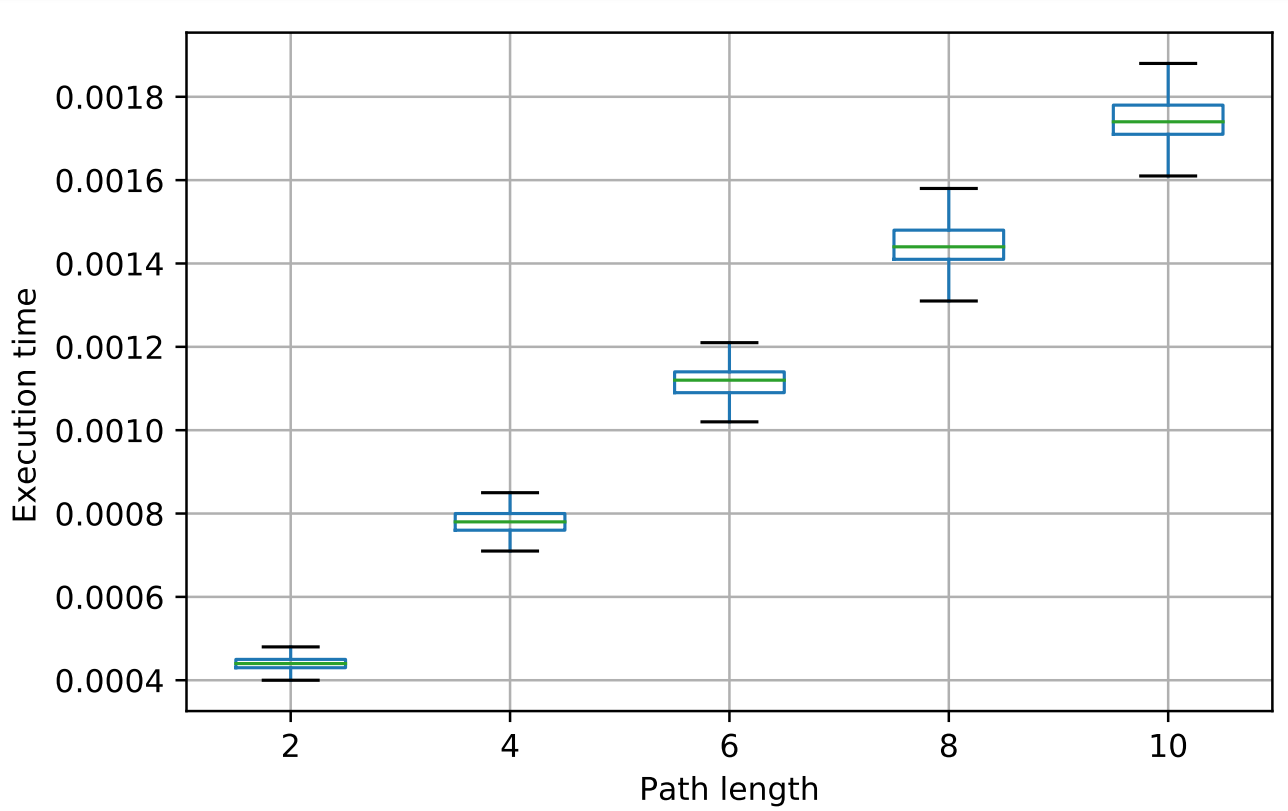
\includegraphics[width=0.62\linewidth]{plots/geo.png}
	\caption{Execution time in seconds of the path extraction algorithm depending on the path length for $geospecies$}
	\label{fig:extractTime}
\end{figure}

We evaluate implementations of devised algorithms on real-world RDFs. We provide results only for our CPU and GPU-based implementations of matrix-based algorithms for relational and single-path query semantics because of the page limit. We use RedisGraph~\cite{8778293} graph database as storage and measure the full time of query execution including all overhead on data preparation. This way we can estimate the applicability of the matrix-based algorithm to real-world problems. The source code is available on GitHub\footnote{Sources of matrix-based CFPQ algorithm for the RedisGraph database: \url{https://github.com/YaccConstructor/RedisGraph}. Access date: 27.02.2021.}

%For evaluation, we use a PC with Ubuntu 18.04 installed.
%It has Intel core i7-6700 CPU, 3.4GHz, DDR4 64Gb RAM, and Geforce GTX 1070 GPGPU with 8Gb RAM.

The results of the CFPQ evaluation are presented in \autoref{tbl:tableRDFQ1}. As we can see, our matrix-based algorithm for relational query semantics implemented for RedisGraph is more than 1000 times faster than the one based on annotated grammar implemented for Neo4j~\cite{Kuijpers:2019:ESC:3335783.3335791} and uses more than 4 times less memory.
We can conclude that the matrix-based algorithm is more performant than the state-of-the-art CFPQ algorithms for query evaluation under a relational semantics for real-world data processing.

%Also, we can see, that the GPU version which utilizes sparse matrices is significantly faster than the other implementations. For example, for $geospecies$ it is more than 7 times faster in both relational and single-path scenarios.
%Note, that for GPU versions we include the time required for data transferring and format conversions.

We can conclude, that the cost of computing matrices for single-path query semantics is not high. On average, it is about 2 times slower than for the relational query semantics. The additional running time of the path extraction is presented in \autoref{fig:extractTime} (boxplots are standard, outliers are omitted). As we can see, this time is small and linear in the length of the path.

Finally, we conclude that the matrix-based algorithm paired with a suitable database and employing appropriate libraries for linear algebra operations is a promising way to make CFPQ with different query semantics applicable for real-world data analysis.
%We show that the SuiteSparse-based CPU implementation is performant enough to be comparable with GPU-based implementations on real-world data.


\section{Conclusion and next steps}
In this Ph.D. work, we provide an approach to solving the CFPQ problem using linear algebra operations. Using provided approach we devise the CFPQ algorithms for all three query semantics and implement them using appropriate libraries for linear algebra operations. Preliminary results show that our CPU and GPU-based implementations that utilize sparse matrix representation and parallel computation outperform the state-of-the-art solutions.

As a next step, we plan to provide a full comparison of our linear algebra-based implementations with all state-of-the-art solutions for CFPQ on the same benchmark and experimental setup. Moreover, our implementations are prototypes and we
plan to provide full integration of CFPQ to RedisGraph. Also, we plan to improve the dataset by including more real-world cases with larger graphs, for example, from the area of static code analysis~\cite{Zheng, veduradabatch}.

\begin{acks}
	This work was funded by RFBR, project number
	19-37-90101, and grant from JetBrains Research.% We also thank [...] for contributing [...].
\end{acks}

%\clearpage

\bibliographystyle{ACM-Reference-Format}
\bibliography{CFPQ_phd_to_VLDB}

\end{document}
\endinput
